\chapter{Experiments and Results}
\label{results}

This section describes the design of the experiments related to the use of fully homomorphic encryption in HElib, as well as a summary of the results obtained. The objective of the experimental design was to test whether or not homomorphic encryption were practical enough to be applied in the cloud as a web application. The feasibility of application in the web depends heavily on the time required to perform homomorphic evaluations, which is affected by several factors. One of these main factors is the \emph{security parameter} $k$, which is a value closely related to the generation of public and private keys and how secure they are. The experimental design consists in changing the $k$ parameter to different values, as to see to what degree it has impact on the key generation, encryption, decryption and addition \emph{processing times}, as well as the \emph{size} of the resulting public key and ciphertext. Finally, the results obtained are presented and briefly discussed. 

\section{Setup}

The experiment is performed by running several iterations of the program that runs in the underlying client-server architecture. To evaluate how the security parameter $k$ affects the time required for certain activities in the software, such as key generation, encryption, decryption, and homomorphic addition of ciphertext. The security parameter $k$ is considered important because the value affects how secure the resulting keys and ciphertexts become. In the design document by Halevi and Shoup \cite{cryptoeprint:2014:106}, it does not specify to what degree changing the value of $k$ would make the cipher vulnerable to cryptanalysis or a brute-force attack; however, it does specify that the technique they propose uses a \emph{ciphertext packing} circuit that can be evaluated homomorphically in time $T \cdot $polylog($k$).

To show how the $k$ security parameter affects the operation of the homomorphic encryption program, the experiment considers several values, namely: 20, 40, 80, 100; where 80 is the default value found in the examples of the HElib. Each value is seen as a \emph{treatment} in the experimental design. For each treatment, the program is run through \textbf{20 iterations} of key generation, encryption, decryption and addition. 

In order to perform the necessary iterations, certain parts of the code from both the client and server sides were taken and adjusted, so that all the operations were performed on the same program. Consequently, overhead operation costs such as sending data between the client and server are not considered for this experiment.

When generating the public and private keys, all of the other parameters are kept \emph{intact}, so that it is only the $k$ value that gets changed. Consequently, the other mechanisms slightly vary because they make use of the previously generated public key.

It is important to consider that the experimentation was done on a notebook which had an AMD Elite A4-5150M processor. The processor is dual core and it runs at 2.7 GHz. Therefore, the results might differ depending on the processor used. Implementation and experimentation of the client-server homomorphic counter solution were done on GNU Linux in the Xubuntu 14.04 distribution.

\section{Results}

The results are presented in Table \ref{tbl:results}, where the column represents the characteristic or attribute considered, such as the processing times and the size of the public key and ciphertext files measured in bytes. Consider that the values presented are the averages obtained from the set of iterations run.

\begin{table}[t]
  \caption{Experimental results}
  \label{tbl:results}
\begin{tabular}{lrrrrrr}
k   & Key Gen. & Key Size  & Encryption & Decryption & Addition & Ctext Size \\
40  & 13.130 s & 165.922 MB & 0.355 s    & 0.048 s    & 0.074 s  & 30.977 kB        \\
60  & 10.710 s & 91.635 MB  & 0.414 s    & 0.056 s    & 0.077 s  & 36.053 kB        \\
80  & 8.380 s  & 57.080 MB  & 0.642 s    & 0.057 s    & 0.082 s  & 37.745 kB        \\
100 & 9.529 s  & 35.453 MB  & 0.579 s    & 0.064 s    & 0.082 s  & 43.676 kB
\end{tabular}
\end{table}

In order to illustrate the differences observed, the following box plot shows the time required to generate the set of keys depending on the size of $k$. It was chosen not to plot the data pertaining to the rest of the attributes under experimentation, mostly because the differences observed were not significant.

\begin{figure}[H]
  \centerline{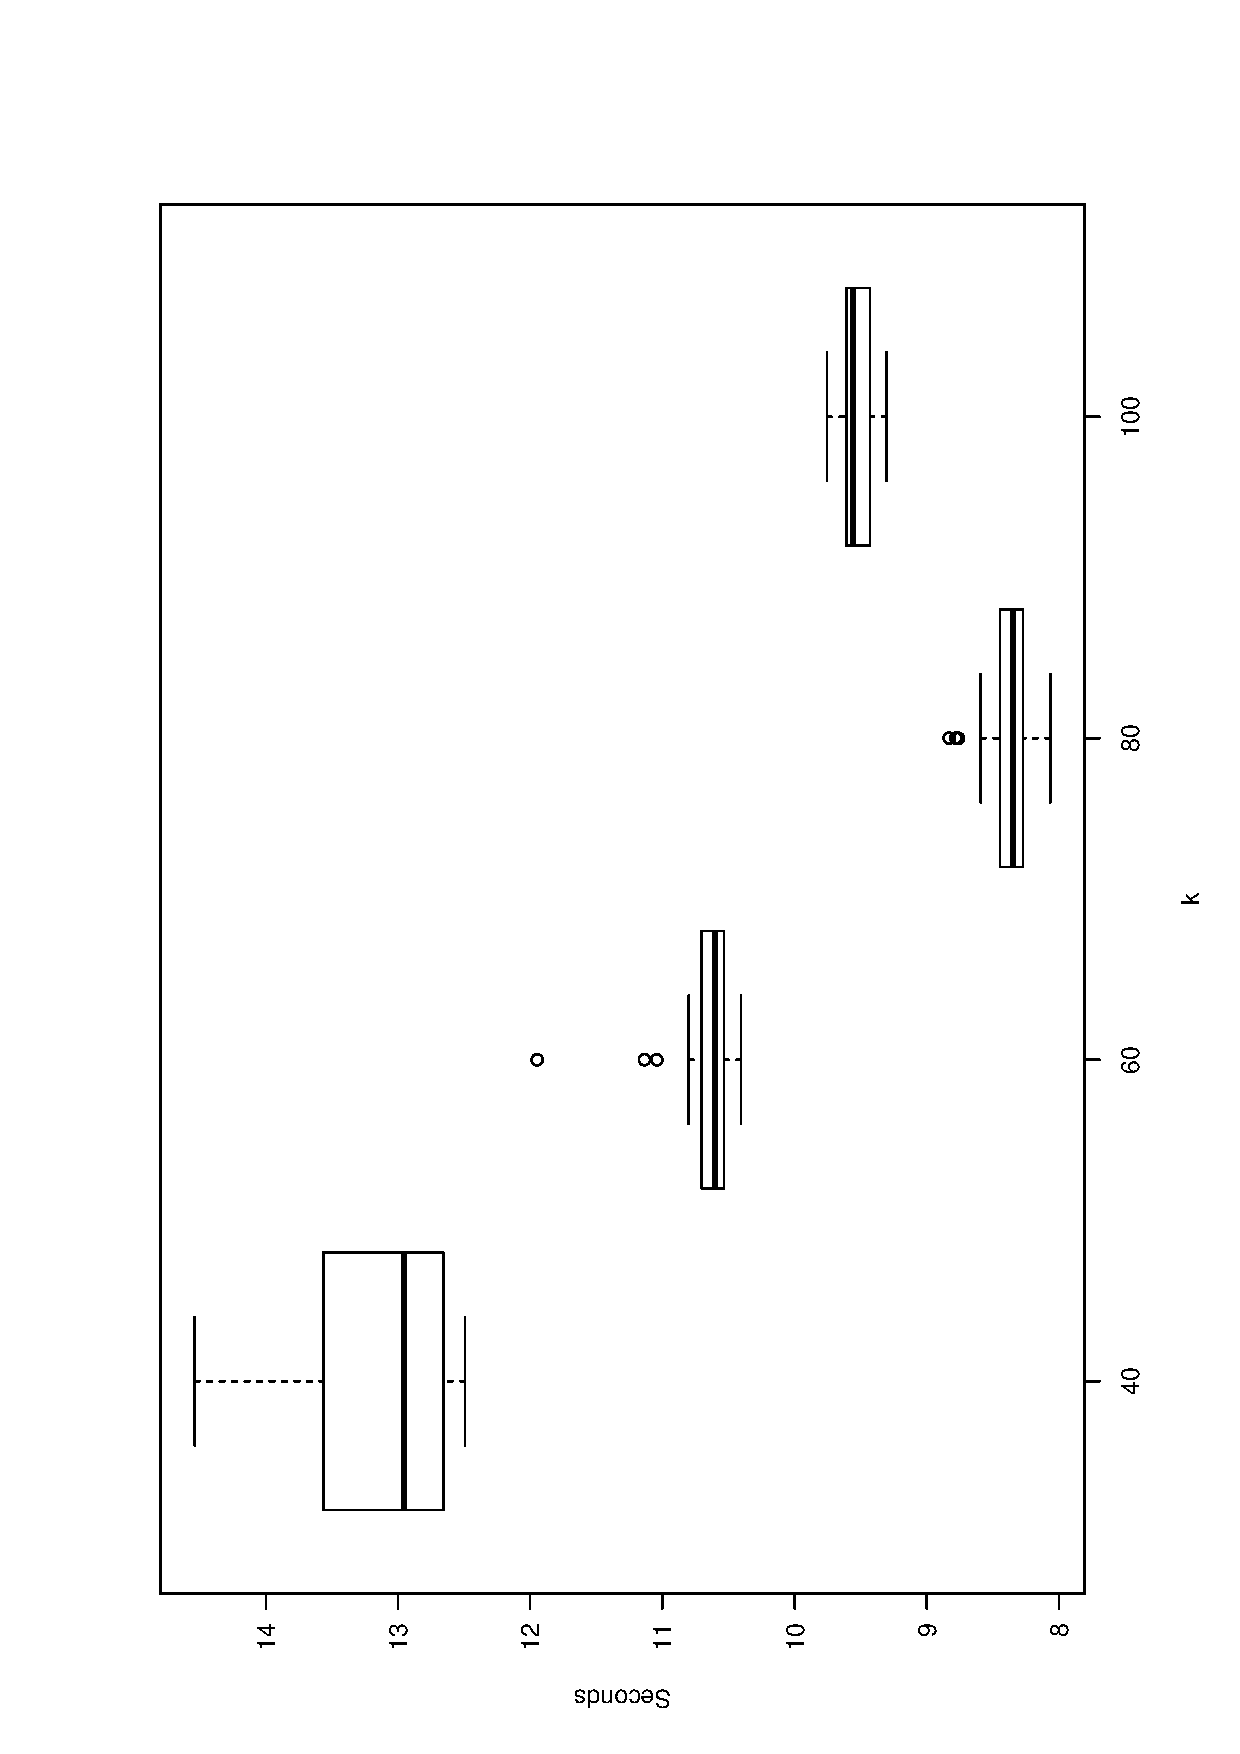
\includegraphics[height=11cm]{img/keygenplot}}
  \caption{Key generation time}
\end{figure}


\section{Discussion}

The first characteristic that is being evaluated is the time needed to generate the set of public and private keys. Usually, the generation of keys is performed only once per user. Only if the private key were compromised, would the user create a new set of keys. Even though 13 seconds, which was the highest average at $k=40$, is relatively a short time. Directly linked to the generation of keys, the size of the key is considered as well. This is because the public key usually has to be shared with others. In this particular case, the averages range between 165.92 at $k=40$  and 35.45 MB at $k=100$. The difference between the sizes is quite large, and even smallest key is significantly large by itself. Additionally, it is puzzling as to why the size of the public key is decreasing as the $k$ parameter gets larger. In cryptography, a larger $k$ usually implies a slowdown in the whole process, but in this case, it does quite the opposite, at least regarding the key generation time.

%Preguntarte si los cambios son poco significativos

Regarding the encryption, decryption, and addition times, the average amount of time required is quite low, and it should not become a bottleneck even if many homomorphic evaluations are performed. Even though the encryption times are longer than the decryption times, none of them surpassed 1 second, which makes it quite acceptable in application. 

Perhaps the most important point to consider is the size of the ciphertexts generated. In the proposed architecture, a ciphertext is constantly sent to the server to perform operations and back to the client for decryption. In the iterations ran, the max average of the ciphertext size was found to be 43.67 kB at $k=100$, while smallest average was 30.99 kB at $k=40$. Looking at how the ciphertext sizes increases, it can be seen that it has a proportional relationship with the security parameter $k$. As $k$ gets larger, so does the size of the ciphertext. This would mean that higher security sacrifices storage, and consequently takes more time to transfer between the client and server.

Even assumming that a security parameter of $k=100$ is used, this shows that the size of the ciphertext is sufficiently small to be used in a web application hosted in the cloud. However, while the client-server architecture program was being developed, an average size of 74 MB per ciphertext was noted. At this time, it is not possible to recreate the scenario where ciphertexts of such a size were created, which leads to the impression that there is another factor not considered that accounts for the size of the ciphertext.

In conclusion, the aforementioned findings suggest that using HElib to apply homomorphic encryption on the cloud might indeed be feasible; however, as it has been noted, there are unknown circumstances that affect the size of the ciphertext. To the best of our knowledge, there is yet no way to predict the size of the ciphertext by using HElib. Therefore, if it is possible to keep the size of the ciphertext below 45kB, then it would certainly be feasible to take this solution to the cloud; otherwise, it would not be possible if each ciphertext had a size that exceded several MB. Until these circumstances are made clear and evaluated properly, it is not possible at this time to show that using HElib to make use of homomorphic encryption in the cloud is indeed feasible. 

% Ver otra manera de poner la ultima oracion

\clearpage
